\item ¿Cuándo fue el último reinicio (Dia, hora y minuto)  de los agentes?

El resultado del último reinicio en Linux como se observa en la figura \ref{image:reinicio} fue:

\FloatBarrier
\begin{figure}[htbp!]
		\centering
	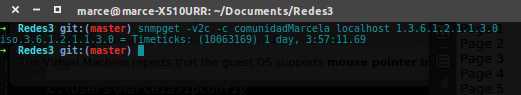
\includegraphics[width=.9 \textwidth]{images/Pregunta1}
		\caption{Último reinicio del agente en Linux con comando snmpget.}
		\label{image:reinicio}
\end{figure}
\FloatBarrier

Por otro lado, el resultado del último reinicio en Windows como se observa en la figura \ref{image:reinicioW} fue:

\FloatBarrier
\begin{figure}[htbp!]
		\centering
			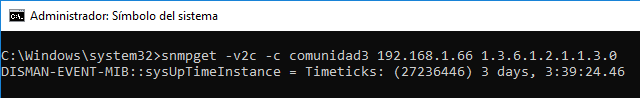
\includegraphics[width=.9 \textwidth]{images/windows1}
		\caption{Último reinicio del agente en Windows.}
		\label{image:reinicioW}
\end{figure}
\FloatBarrier

\item ¿Cuántas interfaces Ethernet tienen?
\\ El resultado en Linux mostrado en la figura \ref{image:interfaces} fue de una interfaz Ethernet.

\FloatBarrier
\begin{figure}[htbp!]
		\centering
	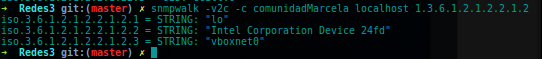
\includegraphics[width=.9 \textwidth]{images/Pregunta2L}
		\caption{Número de interfaces Ethernet en Linux con comando snmpwalk.}		\label{image:interfaces}
\end{figure}
\FloatBarrier

De igual manera, se puede observar en la figura \ref{image:interfacesw} que el resultado en Windows fue de 4 interfaces Ethernet, mostradas a continuación:

\FloatBarrier
\begin{figure}[htbp!]
		\centering
			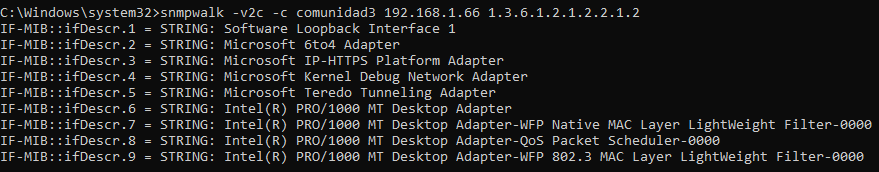
\includegraphics[width=.9 \textwidth]{images/windows2}
		\caption{Número de interfaces Ethernet en Windows.}
		\label{image:interfacesw}
\end{figure}
\FloatBarrier

\item ¿Cuál es la velocidad (en MBPS) de esas interfaces?
\\ El resultado en Linux mostrado en la figura \ref{image:velocidadInterfaces} fue:
\begin{itemize}
\item lo = 100000000
\item Intel Corporation Device 24fd = 0 
\item vboxnet0 = 100000000
\end{itemize}

\FloatBarrier
\begin{figure}[htbp!]
		\centering
			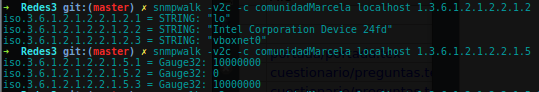
\includegraphics[width=.9 \textwidth]{images/Pregunta3L}
		\caption{Velocidad de las interfaces en Linux con comando snmpwalk.}
		\label{image:velocidadInterfaces}
\end{figure}
\FloatBarrier
Es importante recalcar que en este caso, aunque la interfaz Ethernet corresponder a la llamada ``Intel Corporation Device 24fd'', su velocidad aparece ser de 0 mbps debido a que esta está obteniendo el ancho de banda vía wi-fi y no de forma alámbrica.


En el caso de Windows, el resultado mostrado en la figura \ref{image:velocidadInterfacesw} fue:
\begin{itemize}
\item Software Loopback Interface 1 = 1073741824
\item Microsoft 6to4 Adapter = 0
\item Microsoft IP-HTTPS Platform Adapter = 0
\item Microsoft Kernel Debug Network Adapter = 0
\item Microsoft Teredo Tunnelling Adapter = 0
\item Intel(R) PRO$/$1000 MT Desktop Adapter = 1000000000
\item Intel(R) PRO$/$1000 MT Desktop Adapter$-$WFP Native MAC Layer LightWeight Filter$-$0000 = 1000000000
\item Intel(R) PRO$/$1000 MT Desktop Adapter$-$QoS Packet Scheduler$-$0000 = 1000000000
\item Intel(R) PRO$/$1000 MT Desktop Adapter$-$WFP 802.3 MAC Layer LightWeight Filter$-$0000 = 1000000000
\end{itemize}
\FloatBarrier
\begin{figure}[htbp!]
		\centering
			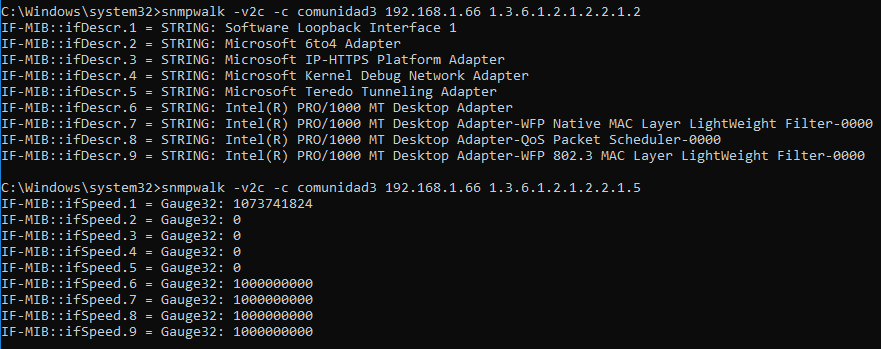
\includegraphics[width=.95 \textwidth]{images/windows3}
		\caption{Velocidad de las interfaces en Windows.}
		\label{image:velocidadInterfacesw}
\end{figure}
\FloatBarrier